\documentclass[10pt,a4paper]{article}
\usepackage[T1]{fontenc}
\usepackage[utf8]{inputenc}
\usepackage{charter}
\usepackage[margin=1.6cm,top=1.45cm,bottom=1.6cm,footskip=0.6cm]{geometry}
\usepackage{microtype}
\usepackage{xcolor}
\usepackage{booktabs,tabularx,array}
\usepackage{enumitem}
\usepackage{titlesec}
\usepackage{tikz}
\usetikzlibrary{positioning,arrows.meta,calc}
\usepackage[hidelinks]{hyperref}
\usepackage{fancyhdr}

\definecolor{navy}{HTML}{1B3A66}
\definecolor{aifill}{HTML}{ECE6FB}\definecolor{ailine}{HTML}{7B5CD6}
\definecolor{codefill}{HTML}{E3EEFB}\definecolor{codeline}{HTML}{3F7CC6}
\definecolor{humfill}{HTML}{FDEEDD}\definecolor{humline}{HTML}{D98A2B}
\definecolor{greyfill}{HTML}{F4F5F8}\definecolor{greyline}{HTML}{9AA2B1}

\titleformat{\section}{\large\bfseries\color{navy}}{\thesection.}{0.5em}{}
\titlespacing*{\section}{0pt}{1.1ex plus .3ex}{0.5ex}
\titleformat{\subsection}[runin]{\normalsize\bfseries\color{navy}}{}{0pt}{}[.]
\titlespacing*{\subsection}{0pt}{0.8ex plus .2ex}{0.5em}
\setlength{\parindent}{0pt}
\setlength{\parskip}{0.45ex}
\setlist{nosep,leftmargin=1.2em,topsep=0.2ex,itemsep=0.15ex}
\renewcommand{\arraystretch}{1.12}
\newcolumntype{L}{>{\raggedright\arraybackslash}X}

\pagestyle{fancy}\fancyhf{}
\renewcommand{\headrulewidth}{0pt}
\fancyfoot[L]{\footnotesize\color{gray}LP Terms Monitor: written brief}
\fancyfoot[R]{\footnotesize\color{gray}\thepage\ / 4}

\newcommand{\code}[1]{\texttt{\small #1}}

\begin{document}

\begin{center}
{\LARGE\bfseries\color{navy} LP Terms Monitor}\\[0.6ex]
{\large Keeping investor reporting deadlines correct after side letters and amendments}\\[0.8ex]
{\small Sandeep Kumar (2023EE30242), IIT Delhi \quad$\cdot$\quad Take-home assignment, November 2026 \quad$\cdot$\quad Area: private fund operations (private equity)\\
All documents used in the prototype are synthetic.}
\end{center}
\vspace{-1ex}

\section{The area, and what surprised me}
A private equity fund is governed by a Limited Partnership Agreement (LPA) that applies to every investor (Limited Partner, LP). Large LPs negotiate \textbf{side letters} that change terms for them alone, for example ``quarterly statements within 45 days instead of the LPA's 60'', an extra ESG report, or monthly cash reporting. Side letters are later changed by \textbf{amendments}. The fund's operations or investor-relations team must deliver every promised report on time, to the right investor, for the life of the fund (often 10+ years). Three things surprised me while reading sample side letters and practitioner guides:
\begin{itemize}
  \item \textbf{Reading the clause is not the hard part; keeping the answer current is.} Amendments rarely restate the obligation. They say things like \emph{``the reference to `forty-five (45) calendar days' in Clause 4.2 is deleted and replaced with `thirty (30) calendar days'\,''}. The true deadline exists only by composing two or three documents in the right order, from the right effective date.
  \item \textbf{``10 business days'' is not a number until you know the calendar.} The LPA's ``Business Day'' definition (e.g.\ London bank holidays) decides the date. Across a year end or Easter, a weekends-only count is 1 to 2 days early, which is a missed deadline.
  \item \textbf{Soft language is deliberate.} ``As soon as practicable'' has no number on purpose. A tool that ``helpfully'' turns it into 30 days creates an obligation nobody agreed to.
\end{itemize}

\section{Problem statement}
\begin{tabularx}{\linewidth}{@{}p{2.1cm}L@{}}
\toprule
\textbf{Who} & Fund operations, investor relations or compliance at a mid-size GP, or the fund administrator acting for it.\\
\textbf{Task} & Maintain a register of every investor-specific reporting obligation (what, to whom, how often, by when), keep it correct as amendments arrive, and show exactly which clause each deadline came from.\\
\textbf{How often} & Bulk work at each fund closing (dozens of side letters at once); ad hoc for each amendment; the resulting deadlines recur monthly and quarterly for every LP for the fund's life.\\
\textbf{Cost today} & Mostly manual abstraction into spreadsheets. Industry guides describe side letter compendiums running to several hundred pages~[1]. My own estimate (an assumption, not validated with a practitioner): 30 to 60 minutes per side letter to abstract and cross-check, plus a re-check on every amendment. The larger cost is the error: a late or missed bespoke report damages the LP relationship, can trigger MFN questions from other LPs, and is the kind of ``did you do what you told investors'' gap regulators examine.\\
\bottomrule
\end{tabularx}

\subsection{Why now}
ILPA's updated Reporting Template (v2.0) was released in January 2025 with implementation from Q1 2026~[2], so reporting packages are being rebuilt and per-LP variations re-examined. The US SEC's Private Fund Adviser Rules, which would have formalised quarterly statements and side letter disclosure, were vacated by the Fifth Circuit in June 2024~[3]; the pressure moved from regulation into LP expectations and examination of disclosures, so GPs carry the tracking burden contractually rather than by rule. In India, SEBI's December 2024 circular and the January 2025 SFA implementation standards now restrict which differential rights AIFs may grant, which makes an accurate inventory of side letter terms a regulatory need there too~[4].

\subsection{Scope}
In scope: periodic \emph{reporting} obligations (deliverable, investor, frequency, deadline, effective date) from LPAs, side letters and deadline-changing amendments; versioning; due-date calculation. \textbf{Out of scope:} deciding legal meaning, validity or precedence between documents (always a human decision); MFN elections; fee and economic terms; event notifications (detected and excluded, not tracked); scanned PDFs and OCR; producing or sending the reports.

\subsection{Jurisdiction}
The synthetic documents follow a common US/Cayman-style PE fund structure with an English-law-style ``Business Day'' definition (London). For another jurisdiction three things change: the holiday calendar (configuration, not code), the document conventions the extraction prompt and regex fast path expect, and the regulatory overlay (for an Indian AIF, e.g., flagging side letter terms outside the SFA positive list of permitted differential rights).

\newpage
\section{Solution design}
\textbf{Core idea:} the AI is allowed to \emph{find and propose}; it is never the source of a number, a date or a decision. Every value it proposes must be literally readable in an exact span of the source document, all arithmetic is done by code, and every change to the register is a human-approved, versioned, audited transaction.

\begin{center}\hyphenpenalty=10000\exhyphenpenalty=10000
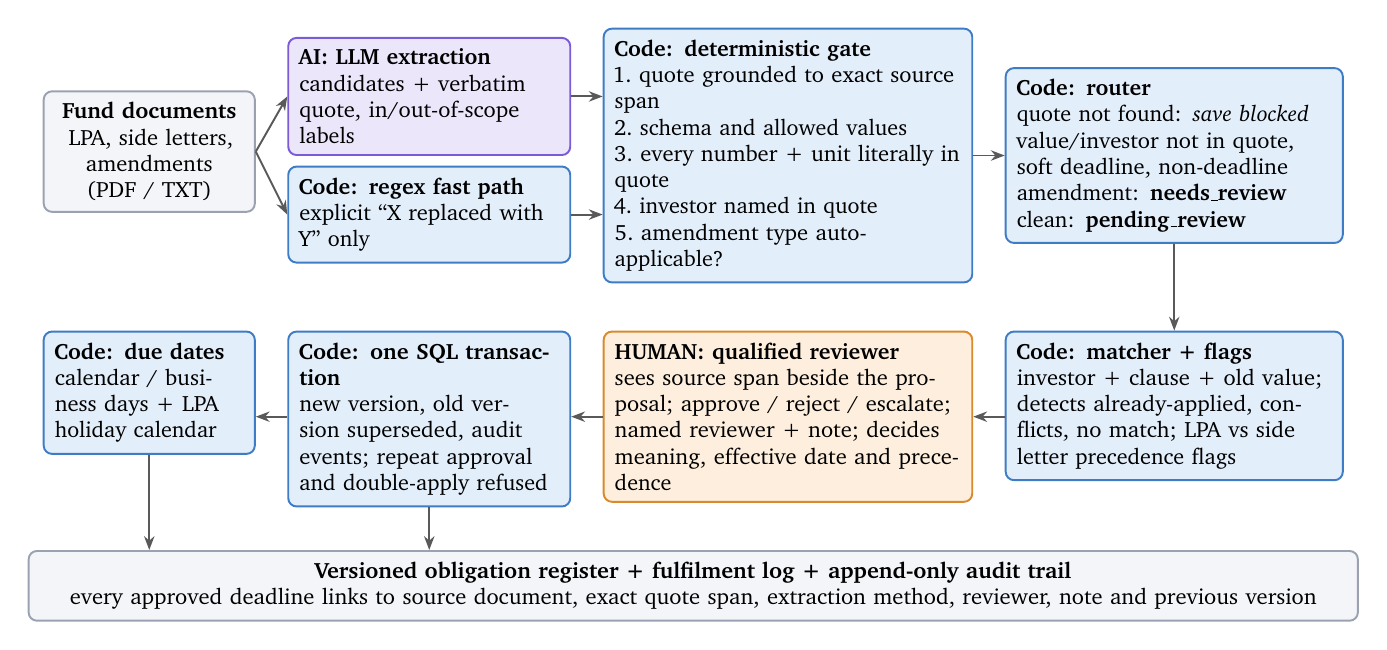
\begin{tikzpicture}[
  font=\footnotesize,
  box/.style={draw, rounded corners=3pt, line width=0.7pt, align=left,  inner sep=4pt, text width=#1},
  ai/.style={box=#1, fill=aifill, draw=ailine},
  cd/.style={box=#1, fill=codefill, draw=codeline},
  hu/.style={box=#1, fill=humfill, draw=humline},
  gr/.style={box=#1, fill=greyfill, draw=greyline},
  arr/.style={-{Stealth[length=5pt]}, line width=0.7pt, draw=black!65},
  node distance=4mm and 4mm]
  \node[gr=2.4cm, align=center] (docs) {\textbf{Fund documents}\\LPA, side letters,\\amendments\\(PDF / TXT)};
  \node[ai=3.3cm, right=4mm of docs, yshift=7mm] (llm) {\textbf{AI: LLM extraction}\\candidates + verbatim quote, in/out-of-scope labels};
  \node[cd=3.3cm, right=4mm of docs, yshift=-8mm] (rx) {\textbf{Code: regex fast path}\\explicit ``X replaced with Y'' only};
  \node[cd=4.4cm, right=4mm of llm, yshift=-7.5mm] (gate) {\textbf{Code: deterministic gate}\\
    1.\ quote grounded to exact source span\\
    2.\ schema and allowed values\\
    3.\ every number + unit literally in quote\\
    4.\ investor named in quote\\
    5.\ amendment type auto-applicable?};
  \node[cd=4.0cm, right=4mm of gate] (route) {\textbf{Code: router}\\
    quote not found: \emph{save blocked}\\
    value/investor not in quote, soft deadline, non-deadline amendment: \textbf{needs\_review}\\
    clean: \textbf{pending\_review}};
  \node[cd=4.0cm, anchor=north east] (match) at ($(route.east |- gate.south)+(0,-6mm)$) {\textbf{Code: matcher + flags}\\investor + clause + old value; detects already-applied, conflicts, no match; LPA vs side letter precedence flags};
  \node[hu=4.4cm, left=4mm of match.north west, anchor=north east] (human) {\textbf{HUMAN: qualified reviewer}\\sees source span beside the proposal; approve / reject / escalate; named reviewer + note; decides meaning, effective date and precedence};
  \node[cd=3.3cm, left=4mm of human.north west, anchor=north east] (tx) {\textbf{Code: one SQL transaction}\\new version, old version superseded, audit events; repeat approval and double-apply refused};
  \node[cd=2.4cm, left=4mm of tx.north west, anchor=north east] (dates) {\textbf{Code: due dates}\\calendar / business days + LPA holiday calendar};
  \node[gr=16.6cm, align=center, anchor=north] (reg) at ($(dates.west |- human.south)!0.5!(match.east |- human.south) + (0,-6mm)$) {\textbf{Versioned obligation register + fulfilment log + append-only audit trail}\\every approved deadline links to source document, exact quote span, extraction method, reviewer, note and previous version};
  \draw[arr] (docs.east) -- (llm.west);
  \draw[arr] (docs.east) -- (rx.west);
  \draw[arr] (llm.east) -- (gate.west|-llm.east);
  \draw[arr] (rx.east) -- (gate.west|-rx.east);
  \draw[arr] (gate) -- (route);
  \draw[arr] (route) -- (match);
  \draw[arr] (match.west|-human.east) -- (human.east);
  \draw[arr] (human.west) -- (tx.east|-human.west);
  \draw[arr] (tx.west|-human.west) -- (dates.east|-human.west);
  \draw[arr] (dates.south) -- (dates.south|-reg.north);
  \draw[arr] (tx.south) -- (tx.south|-reg.north);
\end{tikzpicture}\\[1mm]
{\scriptsize
\tikz\draw[fill=aifill,draw=ailine] (0,0) rectangle (3mm,2mm); probabilistic (AI): may be wrong, never authoritative\qquad
\tikz\draw[fill=codefill,draw=codeline] (0,0) rectangle (3mm,2mm); deterministic (code): exact, tested, auditable\qquad
\tikz\draw[fill=humfill,draw=humline] (0,0) rectangle (3mm,2mm); human: accountable decision}
\end{center}

\vspace{-1ex}
\begin{minipage}[t]{0.485\linewidth}
\subsection{In, AI, out}
\textbf{In:} document text (PDF text layer, TXT, MD) plus optional investor and fund hints. \textbf{AI:} one structured-output call per document returns candidate obligations (or amendment changes) with a verbatim supporting quote, and lists clauses it judged out of scope. \textbf{Out:} a register row only after human approval, with due dates computed by code.

\subsection{Exact vs probabilistic, and how they are kept apart}
The boundary is the database write. Nothing the model returns is stored until the deterministic gate has run, and the stored quote is the \emph{raw source span}, never the model's text. Numbers must be re-readable from that span, as digits or words: ``fifteen Business Days'' passes, an invented 30 days for ``as soon as practicable'' does not. The model's own \code{requires\_human\_review} flag is overwritten to true in code.

\subsection{Why AI is needed at all}
The same obligation is written many ways: numbers in words or digits, sub-paragraph lists, defined terms, deadlines from a period end or from an event. My regex fast path handles the explicit amendment pattern and correctly extracts 4 of my 7 amendment cases, but fails on a line-broken version of the same sentence and cannot express ``extended by a further 15 days''. For side letters, finding deliverable, investor, trigger and deadline in free prose is a language task. The AI earns its place on \emph{recall}; code earns trust on \emph{precision}.
\end{minipage}\hfill
\begin{minipage}[t]{0.485\linewidth}
\subsection{Where knowledge lives, and when it goes stale}
\begin{itemize}
  \item \textbf{Contract terms:} in the stored documents, cited by exact span. An amendment creates a new version; the old one is kept as superseded, so ``what was the deadline on 15 March 2026?'' stays answerable.
  \item \textbf{Counting rules and holiday calendars:} in code and configuration, unit-tested. A changed calendar is a config change, re-tested by the eval.
  \item \textbf{Interpretation:} in human approvals (who, when, note), stored in the audit log.
  \item \textbf{The model:} holds nothing the register relies on. If the model or prompt changes, re-run \code{eval.run\_eval -{}-llm} before use.
\end{itemize}

\subsection{Handling uncertainty and mistakes}
Three outcomes, never silent: \textbf{blocked} (quote not in document), \textbf{escalated} (values not in quote, wrong investor, soft deadline, computed or non-deadline amendment), \textbf{pending} (clean, still needs approval). Escalated amendments are kept for manual handling rather than dropped. Approval re-checks everything inside the transaction and refuses stale matches and double application.

\subsection{Traceability}
Each register row links to its document, exact span, field-level evidence (literal match, inferred from trigger, or explicitly unspecified), extraction method, reviewer and note, and previous version.
\end{minipage}

\newpage
\section{Alternatives considered and rejected}
{\small\begin{tabularx}{\linewidth}{@{}p{4.1cm}L@{}}
\toprule
\textbf{Alternative} & \textbf{Why I rejected it}\\
\midrule
One LLM call that outputs the calendar & No traceability; the model does date arithmetic; nothing stops an invented deadline. Fails ``show me where 30 days comes from''.\\
RAG chatbot over side letters & The problem is \emph{state over time} (which version is in force), not Q\&A. No approval, no history.\\
Second LLM as ``verifier'' & Shares the extractor's failure modes. ``Is the quote real, is the number in it'' is cheaper and exact in code.\\
Fuzzy quote matching & Would accept paraphrases. I normalise only whitespace and quote/dash glyphs, and store the original span.\\
Model applies amendments & ``Extended by 15 days'' needs 75 + 15. Computed contractual values go to a human, never straight to the register.\\
Pure regex; or buy a vendor tool & Regex is kept as a fast path only (it broke on one line break, A03). Commercial tools exist; in practice I would test them against the same verification and versioning bar first.\\
\bottomrule
\end{tabularx}\par}

\section{Prototype and evaluation (17 synthetic documents)}
Streamlit + SQLite app (extraction, register, side-by-side amendment review, lifecycle simulator, audit history; 65 unit tests). My test set: 1 LPA, 9 side letters and 7 amendments with hand-written gold labels, each chosen for a failure mode (words-only deadline, two obligations in one clause, MFN and fee distractors, event trigger, LPA override, unit change, relative change, frequency change, unknown investor, US date format, line breaks). Each gold record is also deliberately broken (invented deadline, paraphrase, re-wrap, unit swap, wrong investor, tampered value) to test whether code catches the model being wrong.

\textbf{\color{navy}Offline result: 102 / 106 checks pass.} All 53 deliberate perturbations were handled correctly (43 injected errors caught, 10 harmlessly re-wrapped quotes accepted). The four failures are real:

{\small\begin{tabularx}{\linewidth}{@{}p{1.4cm}p{5.3cm}L@{}}
\toprule
\textbf{Case} & \textbf{Failure} & \textbf{Why, and what I would do}\\
\midrule
C05, C07 & Business-day due dates 1 to 2 days early with the default weekends-only calendar & Year-end and Easter holidays. Correct once the LPA's London calendar is supplied; production should refuse to compute without one.\\
C07 & Evidence helper cannot locate ``fifteen Business Days'' & Lookup expects digits. The value-in-quote check handles words, so safety holds; the reviewer's evidence panel is incomplete.\\
A03 & Regex fast path declines a line-broken amendment & Falls back to the LLM, which in my runs flattened the line breaks; strict grounding maps the quote back to the raw span. Safe, but model-dependent.\\
\bottomrule
\end{tabularx}\par}

{\small Also: LP-G's sub-paragraph obligations are escalated because the investor is named only in the lead-in sentence, an accepted false positive. Live-model accuracy is scored by the same harness (\code{-{}-llm}); free-tier results vary per run, so they are reported in the repository (\code{eval/results\_llm.md}) rather than claimed here.}

\section{Risks and how the design handles them}
{\small\begin{tabularx}{\linewidth}{@{}p{2.6cm}L@{}}
\toprule
\textbf{Risk} & \textbf{Handling}\\
\midrule
Wrong answers & Precision: the gate; nothing reaches the register without a human. \textbf{Recall is the weak spot} (below).\\
Outdated rules & Amendments create versions with effective dates; superseded versions are kept; duplicate and stale applications are refused. Holiday calendars are versioned config. Model or prompt changes require re-running the eval.\\
Confidential data & Side letters are confidential by contract. Prototype: local, synthetic data only; the free OpenRouter route is for synthetic tests. Production: zero-retention or self-hosted model, encryption at rest, role-based access.\\
Liability, advice & The tool extracts and tracks; it does not interpret. The GP's named reviewer (legal or compliance) is accountable and recorded on every approval. Precedence is flagged, never decided.\\
\bottomrule
\end{tabularx}\par}

\textbf{Weakest point.} The gate checks what the model \emph{found}; it cannot see what the model \emph{missed}, and a skipped clause is exactly how a deadline gets missed. Also likely to break it: deadlines in tables or schedules, cross-references (``the period in Schedule 2''), amendments that restate whole clauses, and reviewers approving by habit. Next fix: a \textbf{coverage check} requiring every sentence with an obligation verb plus a period or frequency to map to a candidate or an explicit exclusion.

\section{Before spending more time on this}
(1) Ask two or three fund operations or administration people whether the pain is first abstraction or keeping up with amendments and MFN elections. (2) Measure recall on real public LPAs and side letters (some public pension plans publish them); synthetic data cannot. (3) Compare vendor tools on recall and audit trail before building more.

\newpage
\section*{Appendix: what I added beyond the AI}

\subsection{Where AI helped}\leavevmode
\begin{itemize}
  \item \textbf{Learning the domain fast:} explaining LPA vs side letter vs amendment, MFN, ILPA templates and ``Business Day'' definitions; I then checked claims against primary or practitioner sources (listed at the foot of this page).
  \item \textbf{Code:} most of the Streamlit UI, SQLite schema and test scaffolding was AI-drafted from my specifications, then reviewed and corrected by me. In the final pass an AI assistant also drafted the value-in-quote consistency check, the precedence flag, the 17-document evaluation harness and a first draft of this brief, from my existing prototype and design decisions.
  \item \textbf{Synthetic documents:} AI drafted clause wording; I chose which failure mode each document should test.
\end{itemize}
\textbf{Key prompts} (the first two are the system prompts the app sends; full chat logs are attached separately):
{\footnotesize\itshape\raggedright
\begin{itemize}[leftmargin=1em,label={\textbullet}]
\item {\upshape\bfseries obligation extraction:} Extract only explicit reporting obligations ... Never infer a deadline that is not explicit. Use null and deadline\_unit='unspecified'. Preserve the exact supporting source\_quote as a verbatim substring. ... Do not decide legal priority between an LPA, side letter or amendment.
\item {\upshape\bfseries amendment extraction:} Extract explicit changes that modify an existing clause ... detect old-value to new-value replacements ... Do not turn an amendment into a new standalone reporting obligation. ... Do not decide whether the amendment is valid, executed, controlling, or legally effective.
\item {\upshape\bfseries to the coding assistant:} The model flattened the line breaks in its quote, so exact matching fails. Do not add fuzzy matching. Normalise only whitespace and quote/dash glyphs to locate the span, then store the original raw span.
\end{itemize}}

\subsection{What I rejected or corrected}\leavevmode
\begin{itemize}
  \item \textbf{Fuzzy matching to ``fix'' quote failures.} Rejected: it would also accept paraphrases, which defeats the point of a citation. I kept strict normalisation and proved with tests that paraphrases fail.
  \item \textbf{Trusting the model's own \code{requires\_human\_review} flag.} Overwritten to true in code: a model cannot be the one that decides it does not need checking.
  \item \textbf{Business days as ``skip weekends''.} Generic and wrong for a contract that defines Business Day; my test cases show 1 to 2 day errors around year end and Easter.
  \item \textbf{``Use a vector database / RAG'' suggestions.} Generic for this problem; the hard part is versioned state and approvals, not retrieval.
  \item \textbf{Letting the model compute amended deadlines} (``extended by 15 days'' becomes 90). Unsafe: a number nobody wrote down would enter the register. Now blocked and routed to a human.
\end{itemize}

\subsection{What came from me}\leavevmode
\begin{itemize}
  \item Framing the problem around \textbf{amendments and versioning} rather than one-off extraction, after seeing that amendments edit a single phrase inside an earlier letter.
  \item The rule \textbf{``store the source span, never the model's words''}, and the gate that numbers must be readable from that span.
  \item A \textbf{narrow deterministic fast path} for the explicit ``deleted and replaced with'' pattern, with the LLM only as a fallback, so the common case is exact and cheap.
  \item A \textbf{separate simulator database} so approve/reject demos never corrupt the real register, and approval implemented as \textbf{one transaction} with stale-match and double-apply checks.
  \item Choosing test documents by failure mode (soft deadline, words-only number, override clause, relative amendment) and reporting the failures rather than tuning them away.
\end{itemize}

\subsection{One thing I would stand behind without AI}
The amendment approval path. An amendment is applied only if it matches exactly one currently approved obligation on investor, clause and old value; the old and new values are literally in the cited amendment text; and the approver is named with a note. In one database transaction the old version is superseded, the new version is created with the amendment's effective date, the candidate is closed and audit events are written. If the register changed since matching (the old deadline is no longer what the amendment says it replaces) or the same amendment was already applied, the transaction refuses. I can explain each check, the failure it prevents, and the test that proves it.

\vfill
{\footnotesize\color{black!70}\rule{\linewidth}{0.4pt}\\
\textbf{Sources.} [1] IQ-EQ and Kirkland \& Ellis, \emph{The Fund Manager's Guide to Side Letters}, Jan 2026. [2] ILPA, Reporting Template v2.0 and \emph{Combined Overview of ILPA Templates} (implementation Q1 2026). [3] Hunton Andrews Kurth, ``Fifth Circuit Court of Appeals Vacates SEC Private Fund Adviser Rules'' (decision of 5 June 2024). [4] SEBI circular of 13 Dec 2024 on pro-rata and pari-passu rights; SFA Implementation Standards, 28 Jan 2025 (via ELP and Vaish Associates summaries).}

\end{document}
